% 请确保文件编码为utf-8,使用XeLaTex进行编译,或者通过overleaf进行编译

\documentclass[answers]{exam}  % 使用此行带有作答模块
% \documentclass{exam} % 使用此行只显示题目

\usepackage{xeCJK}
\usepackage{zhnumber}
\usepackage{graphicx}
\usepackage{hyperref}
\usepackage{amsmath}
\usepackage{booktabs}
\usepackage{enumerate}
\usepackage{amssymb}
\usepackage{bm}
\usepackage{listings}

\pagestyle{headandfoot}
\firstpageheadrule
\firstpageheader{南京大学}{高级机器学习}{习题集一}
\runningheader{南京大学}
{高级机器学习}
{习题集一}
\runningheadrule
\firstpagefooter{}{第\thepage\ 页(共\numpages 页)}{}
\runningfooter{}{第\thepage\ 页(共\numpages 页)}{}

% no box for solutions
% \unframedsolutions

\setlength\linefillheight{.5in}

% \renewcommand{\solutiontitle}{\noindent\textbf{答:}}
\renewcommand{\solutiontitle}{\noindent\textbf{解:}\par\noindent}

\renewcommand{\thequestion}{\zhnum{question}}
\renewcommand{\questionlabel}{\thequestion .}
\renewcommand{\thepartno}{\arabic{partno}}
\renewcommand{\partlabel}{\thepartno .}

\begin{document}
\normalsize

\begin{questions}
\question [30] \textbf{机器学习导论复习题(前八章)}

高级机器学习的课程学习建立在机器学习导论课程的基础之上,从事机器学习行业相关科研工作需要较为扎实的机器学习背景知识。下面的题目则对机器学习基础知识进行复习。

\begin{parts}
	\part [10] 在现实中的分类任务通常会遇到类别不平衡问题,即分类任务中不同类别的训练样例数目类别差别很大,很可能导致模型无法学习。(a) 请介绍类别不平衡学习常用的策略。 (b) 假定当前数据集中每个样本点包含了$\left(\boldsymbol{x}_{i}, y_{i}, p_{i}\right)$,其中$\boldsymbol{x}_i, y_i, p_i$分别表示第$i$个样本的特征向量,类别标签,和样本的重要程度,$0 \leq p_{i} \leq 1$。对于SVM,任意误分样本点$\boldsymbol{x}_i$的惩罚用$p_i$代替,请在西瓜书p130页公式(6.35)的基础上修改出新的优化问题,并给出对偶问题的推导。
	
	\part [20] 通常情况下,模型会假设训练样本所有属性变量的值都已被观测到,但现实中往往会存在属性变量不可观测,例如西瓜根蒂脱落了,就无法观测到该属性值,此时问题就变成了有``未观测"变量的情况下,对模型参数进行估计。EM(Expectation-Maximization)算法为常用的估计参数隐变量的方法。(a) 假设有3枚硬币,分别记作A,B,C。这些硬币正面出现的概率分别是$a,b,c$. 进行如下投掷实验:先投掷硬币A,根据其结果选出硬币B或者硬币C,正面选硬币B,反面选硬币C;然后投掷选出的硬币,投掷硬币的结果,出现正面记作1,出现反面记作0;独立地重复n次实验。假设只能观测到投掷硬币的结果,不能观测投掷硬币的过程。问如何估计三硬币正面出现的概率。请基于EM算法思想详细地写出E步和M步的推导步骤。(b)经典的聚类算法K-means就是EM算法的一种特殊形式,K-means也被称为hard EM。请使用EM算法的思想解释K-means,并对比K-means和EM算法的不同之处。
\end{parts}

\begin{solution}
	\begin{parts}
		\part (a):常用策略有“欠采样”,“过采样”,“阈值移动”等。\\
			  “欠采样”:指的是,在正反例数量不平衡的情况下,采取减少一些反例的方法来进行平衡,之后再进行学习\\
			  “过采样”:与欠采样不同的是采用增加正例的方式来进行平衡,之后再进行学习\\
			  “阈值移动”:假设正例数目为$n^+$,反例数目为$n^-$,分类函数为$y$\\
			  先让模型基于原数据进行学习,在预测类别的时候基于$\frac{y}{1-y} \times \frac{n^-}{n^+} \ge 1 $对样本进行分类\\
			  (b):
			  那么,根据西瓜书p130页公式(6.35)有优化问题:
			  \begin{align*}
			  	&\min_{w,b} \frac{1}{2} ||w||^2 + \sum_{i=1}^{m} p_i \xi_i \\
			  	s.t. &\xi_i \ge 0, i = 1,2,...,m \\
			  	&y_i(w^T x_i + b) \ge 1-\xi_i
			  \end{align*}
		  	  对偶问题转化:
		  	  \begin{align*}
		  	  	L(w,b,\alpha,\mu,\xi) &=  \frac{1}{2} ||w||^2 + \sum_{i=1}^{m} p_i \xi_i + \sum_{i=1}^m \alpha_i (1-\xi_i -y_i(w^T x_i + b)) - \sum_{i=1}^m \mu_i \xi_i\\
		  	  	\frac{\partial L}{\partial w} &= w - \sum_{i=1}^m \alpha_i y_i x_i\\
		  	  	\frac{\partial L}{\partial b} &= \sum_{i=1}^m \alpha_i y_i\\
		  	  	\frac{\partial L}{\partial \xi_i} &= p_i - \alpha_i -\mu_i \\
		  	  \end{align*}
	  	  	  令各项偏导为零可知:
	  	  	  \begin{align*}
	  	  	  	w &= \sum_{i=1}^m \alpha_i y_i x_i\\
	  	  	  	\sum_{i=1}^m \alpha_i y_i &= 0 \\
	  	  	  	p_i &= \alpha_i + \mu_i
	  	  	  \end{align*}
	  	  	  所以代入后问题转换为
	  	  	  \begin{align*}
	  	  	  	L(w,b,\alpha,\mu,\xi) &= \frac{1}{2} \sum_{i=1}^m \sum_{j=1}^m \alpha_i \alpha_j y_i y_j x_i^T x_j + \sum_{i=1}^m (\alpha_i + \mu_i) \xi_i + \sum_{i=1}^m 
	  	  	  	\alpha_i - \sum_{i=1}^m \alpha_i \xi_i - \\ & \sum_{i=1}^m \alpha_i y_i (\sum_{i=1}^m \alpha_i y_i x_i)^T x_i + b \sum_{i=1}^m \alpha_i y_i - \sum_{i=1}^m \mu_i \xi_i \\
	  	  	  	&= \sum_{i=1}^m \alpha_i - \frac{1}{2} \sum_{i=1}^m \sum_{j=1}^m \alpha_i \alpha_j y_i y_j x_i^T x_j
  	  	  	  \end{align*}
			  所以对偶问题是:
			  \begin{align*}
			  	&\max_{\alpha} \sum_{i=1}^m \alpha_i - \frac{1}{2} \sum_{i=1}^m \sum_{j=1}^m \alpha_i \alpha_j y_i y_j x_i^T x_j \\
			  	s.t. &\sum_{i=1}^m \alpha_i y_i = 0 \\
			  	&0\le \alpha_i \le \xi_i
			  \end{align*}
		  	 
		\part (a):
				把最终的观测结果设为$y = (y_1,y_2,...,y_n)$,中途硬币A的投掷结果设为隐变量$z$,构建模型的参数$\theta = (a,b,c)$\\
				对于第i次投掷硬币的结果,可以推出概率表达式:
				\begin{align*}
					p(y_i|\theta) &= \sum_z p(z|\theta) p(y_i|\theta, z) \\
					&= a b^{y_i} (1-b)^{1-y_i} + (1-a) c^{y_i} (1-c)^{1-y_i} 
				\end{align*}
				\begin{align*}
					p(y_i,z = 0| \theta) &= (1-a) c^{y_i} (1-c)^{1-y_i}\\
					p(y_i,z = 1| \theta) &= a b^{y_i} (1-b)^{1-y_i}\\
					p(z=0 | y_i,\theta) &=  \frac{p(y_i,z = 0| \theta)}{p(y_i|\theta)} = \frac{(1-a) c^{y_i} (1-c)^{1-y_i}}{a b^{y_i} (1-b)^{1-y_i} + (1-a) c^{y_i} (1-c)^{1-y_i} }\\
					p(z=1 | y_i,\theta) &= \frac{p(y_i,z = 1| \theta)}{p(y_i|\theta)} = \frac{a b^{y_i} (1-b)^{1-y_i}}{a b^{y_i} (1-b)^{1-y_i} + (1-a) c^{y_i} (1-c)^{1-y_i}}
				\end{align*}
			    为了方便,令
			    \begin{align*}
			    	p(z=1 | y_i,\theta) = 1 - \gamma_i \\
			    	p(z=0 | y_i,\theta) = \gamma_i
			    \end{align*}
		    	则$Q$函数可求得:
		    	\begin{align*}
		    		Q(\theta^{(0)}) &= \sum_{i=1}^n [p(z=0 | y_i,\theta) \ln p(y_i,z = 0| \theta) + p(z=1 | y_i,\theta) \ln p(y_i,z = 1| \theta)] \\
		    		&=  \sum_{i=1}^n \gamma_i  \ln a b^{y_i} (1-b)^{1-y_i} + (1-\gamma_i) \ln (1-a) c^{y_i} (1-c)^{1-y_i} 
		    	\end{align*}
	    		到这里,EM算法的E步求取隐变量的概率分布也就完成了\\
	    		接下来进行M步计算:
	    		\begin{align*}
	    			\theta^1 = \arg \max_\theta Q(\theta^{(0)})
	    		\end{align*}
	    		\begin{align*}
	    			\frac{\partial LL(\theta)}{\partial a} &= \sum_{i=1}^n  \gamma_i \frac{b^{y_i} (1-b)^{1-y_i}}{a b^{y_i} (1-b)^{1-y_i}} + (1 - \gamma_i) \frac{-c^{y_i} (1-c)^{1-y_i}}{(1-a) c^{y_i} (1-c)^{1-y_i}} \\
	    			&= \sum_{i=1}^n \frac{\gamma_i}{a} - \frac{1-\gamma_i}{1-a} \\
	    			&= \sum_{i=1}^n \frac{(1-a)(\gamma_i) - a(1-\gamma_i)}{a(1-a)} \\
	    			&= \sum_{i=1}^n  \frac{\gamma_i - a}{a(1-a)} \\
	    			\frac{\partial LL(\theta)}{\partial b} &= \sum_{i=1}^n \gamma_i \frac{a y_i b^{y_i-1} (1-b)^{1-y_i} - ab^{y_i} (1-y_i) (1-b)^{-y_i}}{a b^{y_i} (1-b)^{1-y_i}} \\
	    			&= \sum_{i=1}^n \gamma_i \frac{ab^{y_i}(1-b)^{1-y_i} [\frac{y_i}{b} - \frac{1-y_i}{1-b}]}{a b^{y_i} (1-b)^{1-y_i}}\\
	    			&= \sum_{i=1}^n \gamma_i \frac{y_i - by_i - b  + by_i}{b(1-b)}\\
	    			&= \sum_{i=1}^n \gamma_i \frac{y_i - b  }{b(1-b)}\\
	    			\frac{\partial LL(\theta)}{\partial c} &= \sum_{i=1}^n (1-\gamma_i) \frac{(1-a) [y_i c^{y_i-1} (1-c)^{1-y_i} - c^{y_i} (1-y_i) (1-c)^{-y_i}] }{(1-a) c^{y_i} (1-c)^{1-y_i}}\\
	    			&= \sum_{i=1}^n (1-\gamma_i) \frac{(1-a) c^{y_i} (1-c)^{1-y_i} [\frac{y_i}{c} - \frac{1-y_i}{1-c}] }{(1-a) c^{y_i} (1-c)^{1-y_i}} \\
	    			&= \sum_{i=1}^n (1-\gamma_i) \frac{y_i - c  }{c(1-c)}\\ 
	    		\end{align*}
				令各项偏导数为0可以求得:
				\begin{align*}
					\frac{\partial LL(\theta)}{\partial a} &= 0\\
					\sum_{i}^n \frac{\gamma_i^{(0)} }{a(1-a)} &= \sum_{i}^n \frac{a}{a(1-a)} \\
					a^{(1)} &= \frac{1}{n} \sum_{i}^n \gamma_i^{(0)} 
				\end{align*}
				\begin{align*}
					\frac{\partial LL(\theta)}{\partial b} &= 0\\
					\sum_{i}^n \frac{\gamma_i^{(0)}  y_i}{b(1-b)} &= 	\sum_{i}^n \frac{\gamma_i^{(0)}  b}{b(1-b)} \\
					b^{(1)} &= \frac{\sum_{i}^n \gamma_i^{(0)}  y_i}{\sum_{i}^n \gamma_i^{(0)} }
				\end{align*}
				\begin{align*}
					\frac{\partial LL(\theta)}{\partial c} &= 0\\
					\sum_{i}^n \frac{(1-\gamma_i^{(0)} ) y_i}{c(1-c)} &= 	\sum_{i}^n \frac{(1-\gamma_i^{(0)} ) c}{c(1-c)} \\
					c^{(1)} &= \frac{\sum_{i}^n (1-\gamma_i^{(0)} ) y_i}{\sum_{i}^n (1-\gamma_i^{(0)} )}
				\end{align*}
				至此,第一轮参数更新就完成了。\\
				按照上述过程继续迭代更新参数直至收敛即可完成EM算法的流程。\\
			  (b):
			  对于K-means算法而言,其中EM算法的E步与K-means算法中对于每一个点$x_i$找到其最近的聚类中心点$\mu_{y_i}$是等价的\\
			  EM算法的M步与K-means算法中的求新的聚类中心点是等价的\\
			  K-means与EM算法的不同在于K-means算法的过程是在给每一个observation分配一个聚类类别,而EM算法的运作过程是在寻找一个聚类类别的似然函数\\
			  并且K-means对于类别的分类是hard的,是一种0-1选择,但是EM算法得出的是一个概率分布,举个例子而言就是可能有0.3的概率分配给$C_1$类,可能有0.7的概率分配给$C_2$类\\
	\end{parts}
\end{solution}


\question [25] \textbf{主成分分析}

主成分分析(Principal Component Analysis, PCA)是一种经典的无监督降维技术,可以有效减少数据维度,避免维度灾难。实际上,涉及PCA的算法有非常多,下面的题目将逐步引入更多关于PCA的内容。

\begin{parts}
	\part [5+5] 关于PCA,教材中给出了最近重构性和最大可分性两种推导方法,但是该方法将多个主成分在一起推导。实际上,有另外一种Step-by-step的推导方法更为具体。假设数据矩阵$X\in \mathcal{R}^{n\times d}$包含$n$个$d$维度的样本,每个样本记作$x_i \in \mathcal{R}^d$。下面基于Step-by-step的最大可分性进行推导。最大可分性的假设偏好是:样本在低维空间尽可能分散。(a) 假设选取第一个主成分为$w \in \mathcal{R}^d$,需要满足$\lVert w \rVert_2^2 = 1$,那么样本投影到该主成分的投影点为$w^Tx_i$,然后我们需要最大化投影点之间的方差,试写出具体的优化目标,并分析其与瑞利商(Rayleigh quoient)的关系。可假设数据已经中心化。(b) 在选取第一个主成分$w$之后,需要求解第二个主成分$v$,要满足和第一个主成分向量正交,即$v^Tw=0$,此时可以考虑将样本$x_i$分解为两个成分:沿着$w$的向量和垂直于$w$的向量。最后只需要对于垂直的部分选取第二个主成分即可。试给出具体的分解方法以及后续选取第二个主成分的推导过程。

	\part [5+5] 假设PCA得到的映射矩阵(主成分组成的矩阵)为$W\in \mathcal{R}^{d \times d^{\prime}}$,那么对数据矩阵$X\in \mathcal{R}^{n\times d}$降维的过程是:$XW \in \mathcal{R}^{n \times d^{\prime}}$。该过程可以看作是神经网络中不带有偏置(bias)的一层全连接映射。那么:(a) 基于最近重构性的PCA推导方法和AutoEncoder有什么关系?试分析二者的区别和联系(可以从公式、优化、实验效果等角度进行分析)。(b) 一般地,在深度神经网络中,对于全连接层会加入正则化项,例如二范数正则化$\lVert W \rVert_2^2$,在PCA中是否可以同样地对$W$施加正则化项呢?试给出具体的优化目标以及大概如何求解。(可参考Sparse PCA相关内容,只需说出求解优化问题的方法,无需给出具体求解算法和过程)。

	\part [5] (任选一题) 上题谈到了PCA和深度神经网络,我们知道深度神经网络一般基于梯度自动回传来进行反向传播,其自动梯度计算过程在PyTorch、Tensorflow等工具包中已经被实现。试问:(a) 请调研sklearn中实现的SVD的方法,试比较其提供的FullSVD、TruncatedSVD、RandomizedSVD等SVD的区别,如果有实验效果对比图(性能、运行效率)则更佳。(b) 试问在PyTorch中是否可以对SVD进行自动计算梯度,如有,请简单介绍其原理。
\end{parts}

\begin{solution}
	\begin{parts}
		\part (a):
		最大化投影点之间的方差可以得知
		\begin{align*}
			\max Var( \bm{w}^T x_i ) = \max \frac{1}{n} \sum_{i=1}^n (\bm{w}^T x_i - \overline{\bm{w}^T x_i}  )^2
		\end{align*}
		因为数据已经中心化,所以$\overline{\bm{w}^T x_i} = 0$\\
		所以问题转化为
		\begin{align*}
			\max_{||\bm{w}||^2_2 = 1} \frac{1}{n} \sum_{i=1}^n (\bm{w}^T x_i)^2 \\
			\max_{||\bm{w}||^2_2 = 1} \bm{w}^T \bm{X}^T \bm{X} \bm{w} 
		\end{align*}
		因为$||\bm{w}||^2_2 = 1$,所以$\bm{w}^T \bm{w} = 1$\\
		所以上述问题可以等价转换为
		\begin{align*}
			\max_{||\bm{w}||^2_2 = 1} \frac{\bm{w}^T \bm{X}^T \bm{X} \bm{w}}{\bm{w}^T \bm{w}} 
		\end{align*}
		而优化问题的优化目标就是在优化瑞利商的一个等价形式。\\
		(b):
		对于一个样本点$x_i$,可以分解为
		\begin{align*}
			x_i = \bm{w}^T x_i \times \bm{w} + (x_i - \bm{w}^T x_i \times \bm{w})
		\end{align*}
		容易推导得
		\begin{align*}
			\bm{w}^T (x_i - \bm{w}^T x_i \times \bm{w}) = \bm{w}^T x_i - \bm{w}^T x_i \bm{w}^T \bm{w} = 0
		\end{align*}
		因此,样本$x_i$已经分解为了互相垂直的两个部分\\
		那垂直部分为
		\begin{align*}
			\bm{X}^\prime = \bm{X} - \bm{X} \bm{w} \bm{w}^T
		\end{align*}
		那么第二主成分为
		\begin{align*}
			v = \arg \max \frac{v^T \bm{X}^T \bm{X} v}{v^T v}
		\end{align*}
		\part (a):
		基于最近重构性的PCA的优化目的在于使得降维后的样本$x^\prime$与降维前的样本$x$之间的距离最小化。\\
		从公式上看,最近重构性的PCA在优化:
		\begin{align*}
			\min \sum_{i=1}^m ||x^\prime - x||^2_2
		\end{align*}
		而Autoencoder的过程是将一个样本$\bm{X} = (x_1,x_2,...,x_m)$通过encoder转化为$\bm{Y}$,再通过decoder转化为$\mathcal{X}$,其优化目标是让经过encoder-decoder作用之后的$\mathcal{X}$与原始$\bm{X}$之间的距离最小化。\\
		从公式上看,Autoencoder在优化:
		\begin{align*}
			\min ||\mathcal{X} - \bm{X}||^2 
		\end{align*}
		这两个优化问题在本质上其实是等价的。\\
		单单对于降维这个目标来说,可以选择通过encoder就完成降维或者通过encoder-decoder来完成降维。\\
		但是区别在于Autoencoder最终的降维可以处理非线性的部分,而PCA只能进行线性降维,这个特点也会在下面的实验结果中有所体现。\\
		Autoencoder通过一个单独的layer并利用线性的转换函数就可以基本实现PCA的效果,在实验中通过简单的神经网络构建,选择线性函数以及tanh函数作为激励函数。\\
		本实验的降维效果基于S型数据(make\_s\_curve):\\
		原图:\\
		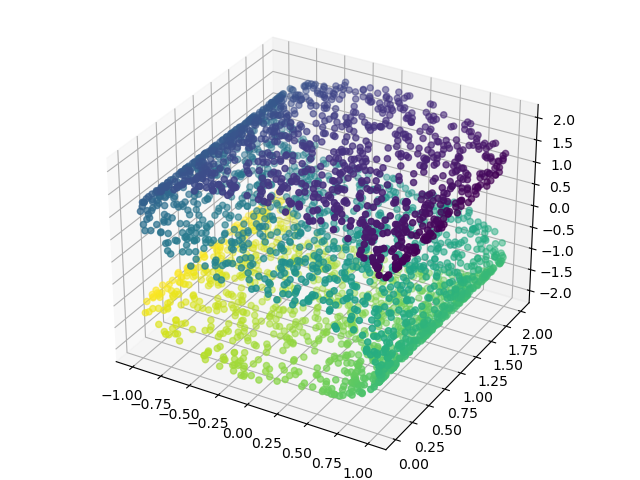
\includegraphics[scale=0.5]{./original_3d_3000.png}\\
		PCA处理之后:\\
		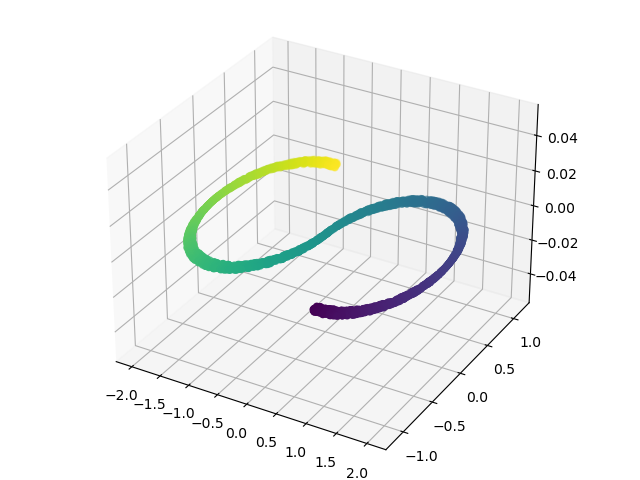
\includegraphics[scale=0.5]{./PCA.png}\\
		AutoEncoder处理之后:\\
		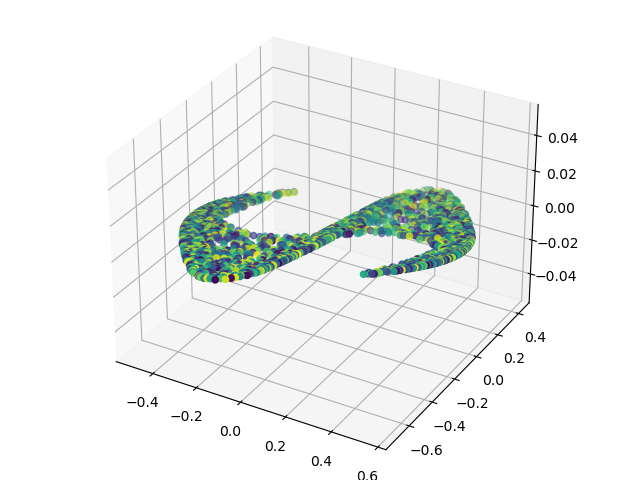
\includegraphics[scale=0.5]{./autoencoder.png}\\
		可见PCA降维处理之后就是一条曲线,而AutoEncoder处理之后就是一个带有曲度的面。\\
		(b):
		在PCA中也可以对$W$施加正则项。\\
		根据Sparse Principal Component Analysis的相关内容可以给出一个具体的优化问题:
		\begin{align*}
			\hat{\beta} = (1+\lambda_2) \arg \min_{\beta} |\bm{Y} - \sum_{j=1}^p \bm{X_j} \beta_j| + \lambda_2 \sum_{j=1}^p |\beta_j|^2 + \lambda_1 \sum_{j=1}^p |\beta_j|
		\end{align*}
		求解这个问题需要用到Sparse Principal Component Analysis这篇paper中提到的算法:\\
		1) : 令$\alpha$为样本数据$\bm{V}$中的前k个主成分\\
		2) : 对于每一个给定的$\alpha$,将上面已经提及的优化问题等价转化为:
		\begin{align*}
			\beta_j = \arg \min_{\beta^*} {\beta^*}^T (\bm{X}^T \bm{X} + \lambda)\beta^* - 2\alpha_j^T  \bm{X}^T \bm{X} \beta^* + \lambda_{1,j} |\beta^*|_1
		\end{align*}
		3) : 对于每一个给定的$\beta$,进行奇异值分解 $\bm{X}^T \bm{X} \beta = U D V^T$,并更新$\alpha = UV^T$\\
		4) : 重复2-3,直到$\beta$收敛\\
		5) : 将结果归一化:$\hat{V_j} = \frac{\beta_j}{|\beta_j|},j=1,...,k$\\
		至此,上述优化问题就可以得到一个通解。
		\part 
		(b):可以,pytorch中通过对于参数$requires\_grad$的设置就可以设定是否需要自动计算梯度。\\
		原理如下:\\
		对于每一个tensor,都有一个属性\.grad\_fn用以记录在反向传播过程中导数的计算方式,并且有属性.is\_leaf来判定是否作为叶子结点在传播过程中进行更新,并且有一个next\_function属性指向下一个运算。\\
		当某个tensor e进行相关运算的时候,就会执行backward(),并且$requires\_grad=True$的时候,系统遍历每一个.is\_leaf为True的叶子,按照.grad\_fn中记录的方法进行更新,并通过next\_function属性将结果送入下一层运算。\\
		因此,当运算结束时,梯度也进行了自动更新。\\
	\end{parts}
\end{solution}

\question [15] \textbf{降维与度量学习}

降维与度量学习包含多种算法,例如PCA、NCA、LLE、MDS等等。接下来的几个题目会拓展大家对这些算法的认知范围。下面三个小题中选做任意两道即可。
\begin{parts}
	\part [5] 近邻成分分析(Neighbourhood Component Anslysis, NCA)是基于KNN分类器的有监督降维算法。其优化目标主要是:$f=\sum_{i=1}^n p_i = \sum_{i=1}^n \sum_{j \in C_i} p_{ij}$,其中$C_i=\{j|y_j=y_i\}$表示与第i个样本类别一样的下标集合,$p_{ij}=\frac{\exp\left(- \lVert Ax_i - Ax_j \rVert_2^2 \right)}{\sum_{k\neq i} \exp\left(- \lVert Ax_i - Ax_k \rVert_2^2 \right)}, j\neq i, p_{ii}=0$表示将第$i$个数据和其余所有样本的近邻概率分布(NN分类过程),距离越近其对应的$p_{ij}$越大,$f$的目标则是最大化留一验证近邻分类的准确性。$A\in \mathcal{R}^{d^\prime \times d}$是待优化的映射矩阵。试推导其梯度$\frac{\partial f}{\partial A}$。
	
	\part [5] 在自然语言处理领域,潜在语义分析(Latent Semantic Analysis, LSA)可以从文档-词矩阵中学习到文档表示、词表示,本质上也是对矩阵进行分解,试查阅相关资料,描述其具体步骤。并简述其与PCA的区别。
	
	\part [5] 根据局部线性嵌入(Locally Linear Embedding, LLE)的算法流程,尝试编写LLE代码,可以基于sklearn实现,并在简单数据集(``S"型构造数据或Mnist等)上进行实验,展示实验结果。
\end{parts}


\begin{solution}
	\begin{parts}
		\part 
		为方便书写,令$\gamma_{ij} = \exp(-||Ax_i - Ax_j||^2_2)$\\
		\begin{align*}
			\frac{\partial f}{\partial A} = \sum_{i=1}^n \sum_{j\in C_i} \frac{\partial p_{ij}}{\partial A} = \frac{1}{(\sum_{k\not= i} \gamma_{ik})^2} [\frac{\partial \gamma_{ij}}{\partial A} \sum_{k\not= i} \gamma_{ik} - \gamma_{ij} \sum_{k\not= i} \frac{\partial \gamma_{ik}}{\partial A}]
		\end{align*}
		\begin{align*}
			\frac{\partial \gamma_{ij}}{\partial A} = -2A \gamma_{ij} (x_i - x_j) (x_i - x_j)^T
		\end{align*}
		代入之后有
		\begin{align*}
			\frac{\partial f}{\partial A} &=\sum_{i=1}^n \sum_{j\in C_i} \frac{1}{(\sum_{k\not= i} \gamma_{ik})^2} [-2A \gamma_{ij} (x_i - x_j) (x_i - x_j)^T \sum_{k\not= i} \gamma_{ik} + \gamma_{ij} \sum_{k\not= i} 2A \gamma_{ik} (x_i - x_k) (x_i - x_k)^T ] \\
			&= \sum_{i=1}^n \sum_{j\in C_i} [\frac{-2A \gamma_{ik} (x_i - x_j) (x_i - x_j)^T}{\sum_{k\not= i} \gamma_{ij}} + \frac{2A \gamma_{ij} \sum_{k\not= i} (x_i - x_j) (x_i - x_j)^T   }{\sum_{h\not= i} \gamma_{ih} \sum_{k\not= i} \gamma_{ik} }] \\
			&= \sum_{i=1}^n \sum_{j\in C_i} [-2A p_{ij}  (x_i - x_j) (x_i - x_j)^T \gamma_{ij} + 2 p_{ij} A (\sum_{k\not= i} p_{ik} (x_i - x_k) (x_i - x_k)^T)] \\
			&= -2A \sum_{i=1}^n \sum_{j\in C_i} p_{ij} [(x_i - x_j) (x_i - x_j)^T- \sum_{k\not= i} p_{ik} (x_i - x_k) (x_i - x_k)^T ]
		\end{align*}
		\part 
		具体步骤:\\
		(1):首先,LSA需要对文档进行分析,构建一个document-term matrix,用来表述terms的出现频率。\\
		(2):其次,LSA希望找到一个document-term matrix的低阶近似来减少计算开销、消除部分噪音、减少一些稀疏性。这一步会将部分表达意思相近的dimensions的信息进行组合表示。\\
		(3):带着这个目的,LSA会对于这个document-term matrix进行建模,用数来表示频率信息,进行奇异值分解,并进行降维操作,完成低阶近似。\\
		(4):对于低阶近似后的结果进行一系列的query、compare,构建一个潜在语义空间,对于每一个query,比较原文与结果所传达出的语义信息。\\
		区别:\\
		(1)LSA是一种明确指定的分析、还原文本的方式,PCA是一种通用的文本分析方式。\\
		(2)在LSA中,上下文主要通过document-term matrix的数字形式传达信息,PCA主要是通过协方差矩阵传达信息。这也表示LSA在寻找一个最佳的线性子空间,而PCA在寻找一个并行的线性子空间。
		\part 
		考虑选用S型构造数据作为dataset,基于sklearn实现lle。\\
		调用S型构造数据需要执行:
		\begin{lstlisting}[language=python]
from sklearn.datasets import make_s_curve
		\end{lstlisting}
		lle方法需要调用sklearn自带的方法:
		\begin{lstlisting}[language=python]
from sklearn.manifold import LocallyLinearEmbedding
		\end{lstlisting}
		对于make\_s\_curve的参数设置如下,并不再进行改变:
		\begin{lstlisting}[language=python]
make_s_curve(n_samples=3000 ,random_state=2021)
		\end{lstlisting}
		先行展示原始三维数据的图形:\\
		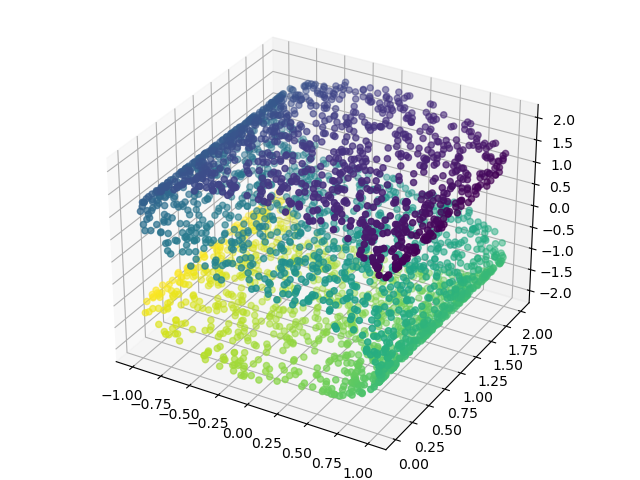
\includegraphics[scale=0.5]{original_3d_3000.png}\\
		在参数为$n\_components=3, n\_neighbors=10, random\_state=2021$的LLE处理之后的图形为:\\
		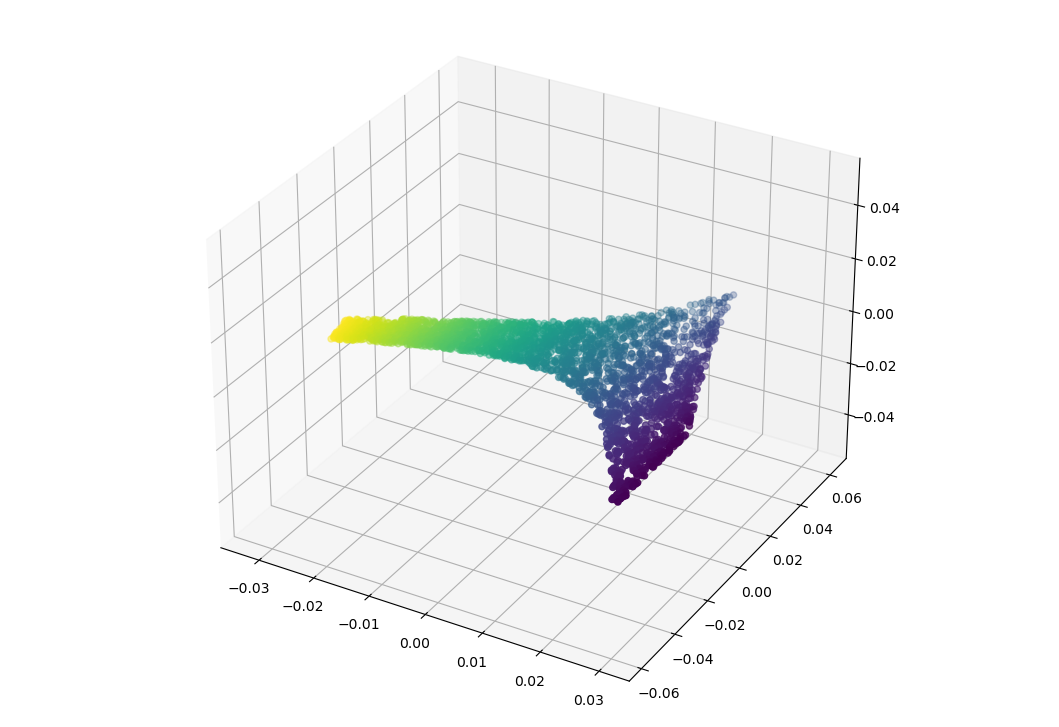
\includegraphics[scale=0.4]{lle_3_10_2021.png}\\
		可以发现降维去除了横向的一维数据。\\
		在换用了the modified locally linear embedding algorithm后,图像发生了明显的平面化:\\
		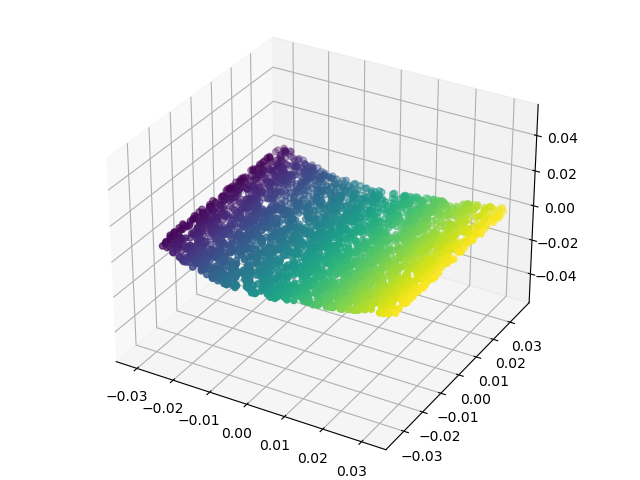
\includegraphics[scale=0.5]{modified.png}\\
		在不改变算法的基础上,更改超参数正则项的值$reg = 1e-2$后,图像也发生了明显的聚集化:\\
		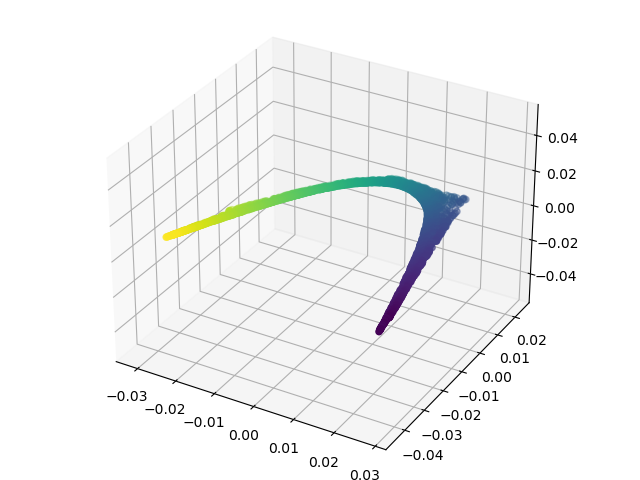
\includegraphics[scale=0.5]{reg_1e2.png}\\
		更改超参数正则项的值$reg = 1e-4$后,图像不再呈现镰刀状\\
		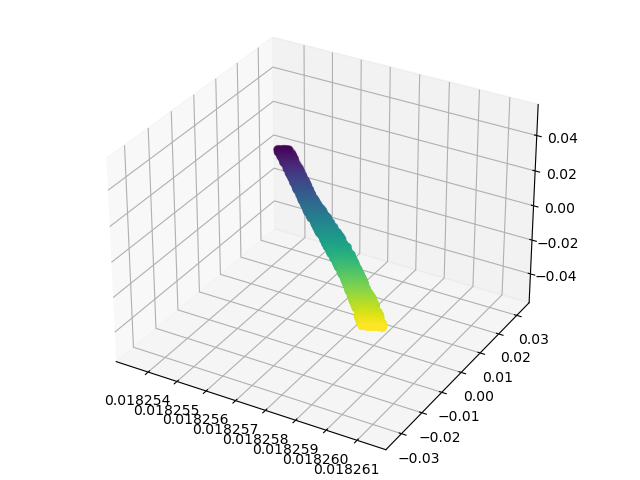
\includegraphics[scale=0.5]{reg_1e4.png}\\
		以上就是对于sklearn中LLE在make\_s\_curve数据集的简单结果展示。\\
	\end{parts}
\end{solution}

\question [15] \textbf{特征选择基础}

Relief算法中,已知二分类问题的相关统计量计算公式如下:
\begin{equation} \delta^{j}=\sum_{i}-\operatorname{diff}\left(x_{i}^{j}, x_{i, n h}^{j}\right)^{2}+\operatorname{diff}\left(x_{i}^{j}, x_{i, \mathrm{nm}}^{j}\right)^{2}
\end{equation}
多分类的Relief-F算法的相关统计量计算公式如下:
\begin{equation}
	\delta^{j}=\sum_{i}-\operatorname{diff}\left(x_{i}^{j}, x_{i, \mathrm{nh}}^{j}\right)^{2}+\sum_{l \neq k}\left(p_{l} \times \operatorname{diff}\left(x_{i}^{j}, x_{i, l, \mathrm{nm}}^{j}\right)^{2}\right)
\end{equation}
其中$p_l$为第$l$类样本在数据集$D$中所占的比例。然而仔细观察可发现,二分类问题中计算公式的后一项$\operatorname{diff}\left(x_{i}^{j}, x_{i, \mathrm{nm}}^{j}\right)^{2}$的系数为1,多分类问题中后一项系数求和小于1,即$\sum_{l \neq k}p_l = 1-p_k < 1$。基于这个发现,请给出一种Relief-F算法的修正方案。


\begin{solution}
	一种朴素的修正方法就是在计算比例时去除第k类的影响:\\
	\begin{align*}
		p_l^\prime = \frac{p_l}{1-p_k}, l\not= k
	\end{align*}
	将修正后的$p_l^\prime$代入到原式当中,可以保证:
	\begin{align*}
		\sum_{l \not= k} p_{l}^{\prime} = \frac{\sum_{l \not= k} p_l}{1-p_k} = 1
	\end{align*}
	此时的$p_l^\prime$仍然可以起到指示第l类样本的猜错近邻在j属性上的作用大小与其他所有可能猜错的类中的比例。\\
	对修改后的$p_l^\prime \times \operatorname{diff}\left(x_{i}^{j}, x_{i, l, \mathrm{nm}}^{j}\right)^{2}$进行求和后,可以在保持系数为1的情况下,反映第k类样本以外的样本的估计平均。\\
\end{solution}

\question [15] \textbf{特征选择拓展}

本题借助强化学习背景,主要探讨嵌入式选择在强化学习中的应用。强化学习可以看作一种最大化奖励(也就是目标)的机器学习方法,目的是学习到一个策略,使得执行这个策略获得的奖励值最大。基于TRPO(一种强化学习方法)的近似方法的近似问题如下
\begin{equation}
	\begin{array}{cc}
		\max\limits_{\theta} & \left(\nabla L_{\theta_{\text {old }}}(\theta)\right)^{T}\left(\theta-\theta_{\text {old }}\right) \\
		\text { s.t. } & \frac{1}{2}\left(\theta-\theta_{\text {old }}\right)^{T} H\left(\theta-\theta_{\text {old }}\right) \leq \delta
	\end{array}
\end{equation}
这里采用了参数化表示方法,其中$\theta$表示新策略,$\theta_{\text {old }}$表示旧策略,方法需要通过策略的目标函数$L_{\theta_{\text {old }}}$来更新旧策略,最终目标是学习到最大化目标函数的新策略。这里要最大化的表达式可以对应理解为最小化损失函数,即类似于课本252页式(11.5)。\\
如果将目标$L$分解为很多个子目标,即$L=\left[L_{1}, L_{2}, \ldots, L_{n}\right]^{T}$,每个目标对应相应的权重$w=\left[w_{1}, w_{2}, \ldots, w_{n}\right]^{T}$,新方法(称为ASR方法)的优化目标如下
\begin{equation}
	\begin{array}{cl}
		\max _{w} & \max _{\theta}\left(\nabla\left(L^{T} w\right)\right)^{T}\left(\theta-\theta_{\mathrm{old}}\right) \\
		\text { s.t. } & \frac{1}{2}\left(\theta-\theta_{\mathrm{old}}\right)^{T} H\left(\theta-\theta_{\mathrm{old}}\right) \leq \delta \\
		& \|w\|_{1}=1 \\
		& w_{i} \geq 0, \quad i=1,2, \ldots, n
	\end{array}
\end{equation}

问:
\begin{parts}
	\part [10] 尝试分析ASR方法中加入$w$的L1范数约束的现实意义。(提示:不同目标对应的参数$w_i$是需要学习的参数。原目标$L$现由多个子目标组成,每个子目标的质量良莠不齐)
	\part [5] 在ASR方法基础上提出的BiPaRS方法解除了$w$的L1范数这一限制,使得更多样$w$可以出现、更多种$L$可以被使用。结合这一点,论述特征选择需要注意的事项。
\end{parts}

\begin{solution}
\begin{parts}
	\part
	(i):如果没有$w$的L1范数约束,单单只有$w_i \ge 0$的约束。\\
	那么对于不同的目标的学习参数$w_i$与$w_j$之间可能出现数值差距过大的情况,不妨假设$w_i >> w_j$,这将使得模型十分注重目标$L_i$的实现情况而极大忽略目标$L_j$的实现情况。\\
	在训练过程中,我们并不知道目标$L_i$与目标$L_j$的质量如何,如果目标$L_i$实际上对于整个模型的学习并没有什么好处但是权值却很大,需要经过大量的学习过程去修正,增加计算开销。\\
	并且这种侧重性可能只是某些训练数据的一个特点,不具有泛化性,这会不可避免地使得模型走向过拟合。\\
	通过引入$w$的L1范数约束,保证每一个$w_i$所起到的作用有限、可控,减少过拟合的可能性。\\
	(ii):另外一方面,引入L1范数约束,使得不同目标的权重之和为1,也增强了模型的可解释性。对于不同的子目标,我们可以清楚地知道,学习的过程就是在优化、调整不同子目标对于整个目标的重要程度。\\
	(iii):L1范数约束会增强稀疏性但又不至于过度稀疏,使得部分的正向子目标的重要性得以有效体现,实现自动选择。\\
	\part
	(i)ASR方法中加入$w$的L1范数约束,但是在BiPaRS方法中又取消了$w$的L1范数约束,而不同的特征选择可以训练出不同的模型应用于不同的问题。就像BiPaRS方法与ASR方法相比,对于不同的子目标就具有更强的包容性,优化目标的多样性也得以提升。\\
	由此可见,对于不同的任务,需要进行灵活的特征选择策略的调整。针对不同问题,进行不同的特征选取策略的选取来使得学习效果更佳。\\
\end{parts}
	
\end{solution}


\end{questions}

\end{document}